\begingroup

\TPGrid{3}{36}
\textblockorigin{0mm}{0mm}
\setlength{\parindent}{0mm}
\setlength{\banderougewidth}{2\TPHorizModule}
\setlength{\banderougeheight}{\TPVertModule}
\setlength{\bandeorwidth}{\TPHorizModule}
\setlength{\bandeorheight}{\banderougeheight}
\setlength{\imageheight}{29\TPVertModule}
\setlength{\imagewidth}{3\TPHorizModule}
\setlength{\logoheight}{2.5\TPVertModule}
\setlength{\gapwidth}{0.75pt}
\addtolength{\bandeorwidth}{-\gapwidth}
\addtolength{\imageheight}{-\gapwidth}

\begin{frame}[plain]
  %% bandeau identitaire
  \begin{textblock*}{3\TPHorizModule}[0,1](0mm,30\TPVertModule)
    \textcolor{rouge}{\rule{\banderougewidth}{\banderougeheight}}% % bande rouge
    \rule{\gapwidth}{0pt}%                                         % filet
    \textcolor{or}{\rule{\bandeorwidth}{\bandeorheight}}           % bande or
  \end{textblock*}

  %% logo UL
  \begin{textblock*}{\TPHorizModule}(2\TPHorizModule,31\TPVertModule)
    \rule{\gapwidth}{0pt}%                                     % filet
    \includegraphics[height=\logoheight,keepaspectratio=true]{ul_p}
  \end{textblock*}

  %% image de fond
  \begin{textblock*}{3\TPHorizModule}(0mm,0mm)
    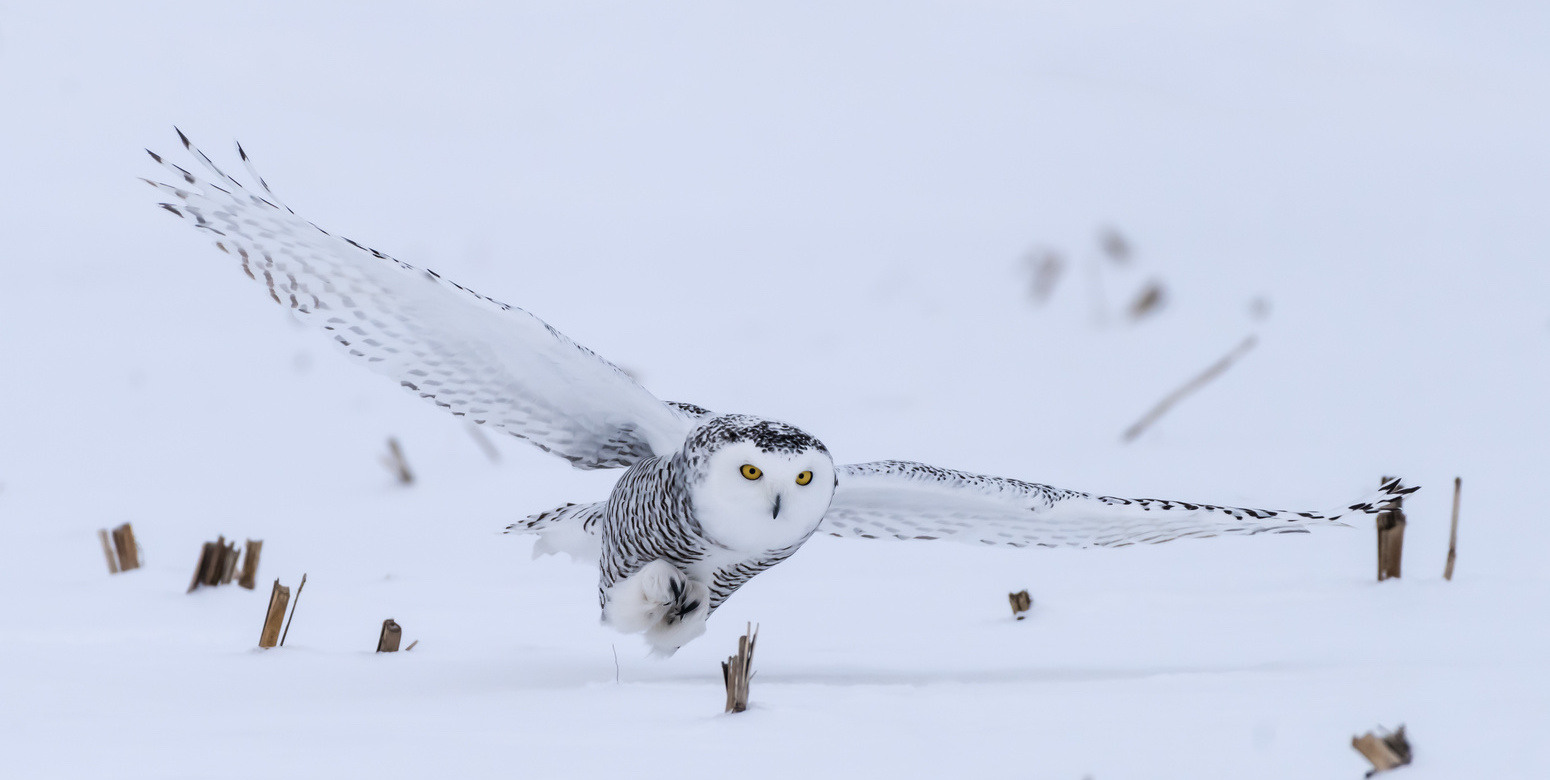
\includegraphics[height=\imageheight,width=\imagewidth]{Fotolia_99831160.jpg}
  \end{textblock*}

  %% titre
  \begin{textblock*}{2\TPHorizModule}(0.2\TPHorizModule,3\TPVertModule)
    \raggedright%
    \bfseries
    \fontsize{30}{30}\selectfont
    Introduction à R \\
    \mdseries
    \fontsize{14}{18}\selectfont
    Atelier du colloque R à Québec 2017
  \end{textblock*}

  %% date
  \begin{textblock*}{2\TPHorizModule}(0.2\TPHorizModule,26\TPVertModule)
    \fontsize{10}{12}\selectfont
    25 mai 2017
  \end{textblock*}
\end{frame}
\endgroup

%%% Local Variables:
%%% mode: latex
%%% TeX-engine: xetex
%%% TeX-master: "raquebec-atelier-introduction-r"
%%% End:
